% \documentclass[12pt]{article}
% \usepackage{color,soul}
% \usepackage[colorlinks = True,
%             linkcolor = black,
%             urlcolor  = black,
%             citecolor = black,
%             anchorcolor = black]{hyperref}
%
% \usepackage[version=4]{mhchem}
% \usepackage{graphicx}
% \usepackage{array} % for better arrays (eg matrices) in maths
% \usepackage[T1]{fontenc}
% \usepackage[utf8]{inputenc}
% \usepackage{mathptmx}
% \usepackage{cleveref}
% \usepackage{outlines}
% \linespread{1.25}
% \usepackage[parfill]{parskip}
% \usepackage[top=1in, bottom=1in, left=1in, right=1in]{geometry}
% \geometry{letterpaper}
%
% \usepackage[numbers]{natbib}

\documentclass[a4paper,num-refs]{oup-contemporary}

\journal{gigascience}

\usepackage{graphicx}
\usepackage{siunitx}



\title{Keeping it light: (Re)analyzing community-wide datasets without major infrastructure}

\author[1]{Harriet Alexander}
\author[1]{Lisa K. Johnson}
\author[1,\authfn{1}]{C. Titus Brown}

\affil[1]{Population Health and Reproduction, University of California, Davis, CA, USA}

%%% Author Notes
\authnote{\authfn{1}titus@idyll.org}


\papercat{Commentary}

\runningauthor{Alexander et al.}

\jvolume{00}
\jnumber{0}
\jyear{2018}


\begin{document}

\begin{frontmatter}
\maketitle

  \begin{abstract}
    Sequencing technology has revolutionized the field of biology, shifting biology from a data-limited to data-replete state. Central to the interpretation of sequencing data are the computational tools and approaches that convert raw data into biologically meaningful information. Both the tools and the generation of data are actively evolving, yet the practice of re-analysis of previously generated data with new tools is not commonplace. Re-analysis of existing data provides an affordable means of generating new information and will likely become more routine within biology, yet necessitates a new set of considerations for best practices and resource development. Here, we discuss several practices that we believe to be broadly applicable when re-analyzing data, especially when done by small research groups.

  \end{abstract}

\begin{keywords}
reproducibility; data reuse; open data;
\end{keywords}
\end{frontmatter}

\section{Background}
Advances in high-throughput, next-generation sequencing technologies have catapulted biology into a new computational era. In fields of biology that leverage sequencing data, the primary limiting step in the earlier stages of biological inquiry has increasingly shifted away from data generation to data analysis. Concomitant with the increasing emphasis on the computational processing of these data is the advancement of the computational tools available for such analyses: new computational approaches for the analysis of these data are constantly being created, tested, and proved worthy of use. Yet, outside of computational lab groups, the practice of re-analysis of previously generated data with new tools and approaches is not commonplace. Such re-analysis has great utility and will become more routine within the life sciences, yet re-analysis necessitates a new set of considerations for best practices and resource development.


%The field, of biology, however lacks a set of agreed upon best practices for the reanalysis of biological data.
% these new tools and improved software are published and gain recognition, new biological insights stand to be gained from the reanalysis of these archived data.

Our interest in the issues surrounding re-analysis was spurred by a large-scale sequencing project: the Marine Microbial Transcriptome Sequencing Project (MMETSP), which generated 678 transcriptomes, spanning 396 different strains of eukaryotic microbial eukaryotes isolated from marine settings \cite{Caron2016}. This dataset is an invaluable resource within the oceanographic community \cite{Keeling2014, Caron2016}, as it exponentially expands the accessible genetic information base of marine protistan life. Moreover, the MMETSP has created a uniquely useful test dataset for computational biologists. The MMETSP dataset spans a large evolutionary history of organisms, and all of the 678 transcriptomes were prepared and sequenced in a consistent way \cite{Keeling2014}. The sequencing project, which was completed in 2014, was originally assembled by the National Center for Genome Resources using a custom pipeline that employed the best available computational tools at the time \cite{Simpson2009, Huang1999}.

Since the original MMETSP analysis, new tools and techniques for the assembly of {\em de novo} transcriptomes from RNAseq data have been described and preexisting tools have been improved upon \cite{Grabherr2011}. Moreover, new annotation tools and databases have become available. The transcriptome assembly project described in \citet{Johnson2018} was designed to create a push-button assembly framework that not only enables the re-analysis of these datasets, but creates a framework to facilitate easy and rapid re-analyses in the future.

These secondary data products of sequencing, such as annotated
assemblies, should be viewed as hypotheses generated from the
underlying biology, rather than some immutable `truth'. As such these
secondary data products can continue to be improved as new tools are
developed.  For example, we note that \citet{MacManes177253} described several
limitations and challenges of current assembly technology and developed
an improved Oyster River Protocol, which we could use to generate another,
perhaps improved, MMETSP assembly.

Ultimately, such iterations on the original raw data have the
potential to improve upon the secondary data products -- the assembled
transcriptomes and associated annotations that are relied upon by the
broader community for biological inquiry. Through this process, we developed several
practices that we believe to be broadly applicable when re-analyzing data,
especially when done by small research groups.


\section{Main text}
\subsection{Storage of secondary data products}
Funding agencies and academic journals now mandate the deposition of raw data into digital repositories (e.g. NCBI Sequence Read Archive (SRA) and Gene Expression Omnibus, European Nucleotide Archive). Thus, to date, the majority of the sequence data that has been generated and published are openly available online for reference and use in other studies. The sharing and availability of raw data from high-throughput sequencing studies has been largely managed through the development of archival services such as the SRA, which was established as part of the International Nucleotide Sequence Database Collaboration (INSDC)\cite{Kodama2012, Shumway2009}. The SRA currently contains more than 1.8e16 bases of information (\textasciitilde7e15 are open access)\footnote{As of 17 May 2018.}. While a tremendous resource for biological inquiry, a major problem remains in that raw sequencing data is not the most directly useful form of sequencing data. Rather, biologists rely heavily upon the computationally generated secondary products of sequencing reads (e.g. assembled transcriptomes or genomes, annotations, associated count-based data, etc.). There is a dearth of these secondary products in central, publicly accessible databases, such as the  Transcriptome Shotgun Assembly (TSA) Sequence Database.

In fact, a substantial proportion of these data products might be aptly categorized as ``dark data,'' as they are largely undiscoverable and often archived independently in association with a publication or on private servers. Even more limiting, however, is that the guidelines for public databases such as the TSA specifically state that ``Assemblies from sequences not directly sequenced by the submitter'' should not be uploaded to the TSA, thereby excluding the potential for reassembled datasets to be made available and directly linked to preexisting BioProjects, BioSamples, TSAs, and SRA entries (https://www.ncbi.nlm.nih.gov/genbank/tsa/).

From the perspective of our MMETSP re-analysis, we argue the community needs more than a place to put the primary and secondary data products associated with a single publication. Ideally, the results of each re-analysis would be deposited in a discoverable location, but would have a coherent archival procedure that is lab-independent, easily searchable, and ``forward discoverable'' (i.e. when a  new version of a data product is released, old versions can point to the new version). Moreover, such an archival platform would ideally document the full provenance of the secondary data product. Movement towards this kind of data archival system are being made both with the development of alternative scientific data publication models (e.g. the Research Object\cite{Bechhofer2013}) as well as integration of metadata models (such as the Resource Description Framework) onto existing scientific databases like the European Bioinformatics Institute (EBI) \cite{Callahan2013}, but policies surrounding secondary data products will need to change.

\subsection{Directly linking secondary data products to provenance of work-flow}


In the absence of a community database specifically for the type of
secondary product that was produced in this analysis, we opted to
upload the assemblies, annotations, and counts to Zenodo
(https://zenodo.org), a scientific data repository founded by CERN,
which provided DOIs for the assemblies (https://doi.org/10.5281/zenodo.746048).
We then created a GitHub
repository containing the scripts used to generate the assemblies, and
added the output data DOIs (\ref{fig:FlowDiagram}).  The entirety of the
repository was then archived with Zenodo, which generated a single DOI
for the project (https://doi.org/10.5281/zenodo.249982).

As such, the scripts used in the generation of transcriptomes are
directly linked through a unique DOI to the data products that are
listed in the directory. Since the scripts are easily accessible, they
can be tweaked to re-analyze the primary sequence data using different
parameters or tools, and the new pipeline and output files can be
archived again with Zenodo using the same approach as above.
Moreover, the Zenodo archival system will then automatically indicate
the presence of other versions of a given repository such that a user
might be sure to use the newest version of an assembly. In the future,
such an approach might be further complemented by the integration of a
JSON Linked Data file detailing the metadata for the assembly product,
such as the pipeline used and previous versions of the assemblies.\footnote{It should be noted that uploading the assemblies to Zenodo was not an automated process. New versions of files on Zenodo must be manually curated. Since the start of this project, the Open Science Framework (OSF) and the accompanying automated command-line client, osfclient has been established. In the future, large-scale projects such as the assemblies created in this analysis will benefit from the integration of OSF command-line client by automatically uploading data products to an OSF project, which generate an OSF-specific DOI.}

\begin{figure}
  \centering
  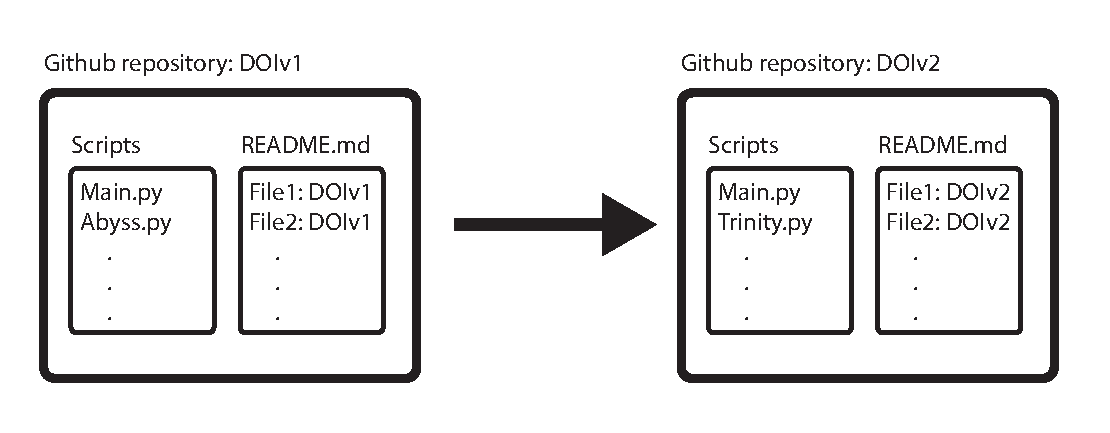
\includegraphics[width=\linewidth]{Diagram.pdf}
  \caption{Flow of coupled script and data product evolution.}
  \label{fig:FlowDiagram}
\end{figure}
\section{Conclusion}

The Github-Zenodo framework presented here represents a relatively low
cost, undemanding way for small research groups (i.e. a graduate
student) to perform large-scale re-analysis projects in an efficient
and publicly accessible way. The direct linking of protocols and
metadata to output data products is paramount in the data heavy future
of scientific advancement. We also identified several lingering issues surrounding large scale
re-analysis.

Actual computation on these large datasets is a non-trivial issue, as
it requires access to facilities with sufficiently large, high-memory
machines.  Amazon Web Service instances and other ``cloud'' platforms,
including XSEDE, provide flexible computing options, and are broadly
accessible. Cloud-based systems, however, tend to be more expensive
per computation hour than local resources. High Performance Computing
(HPC) resources at local institutions represent another potential site
of compute ability.  However, HPCs can be temperamental and
potentially balk at larger, more node-consuming procedures; moreover,
bioinformatics tools may poorly optimized for HPCs: Trinity, used in
our pipeline, creates many small files for each run, and this
repeatedly caused disk slowdowns on our HPC.  The re-analysis by
\citet{Johnson2018} attempted to use both but ultimately
found that the HPC provided the most consistent scalable automation
for running hundreds of jobs in a cost efficient manner.  However,
more generally, we see no global solution for identifying and
optimizing the global scientific cyberinfrastructure requirements for
projects which require significant scaling; such considerations must
be made on a project-by-project basis given the resources available to
each lab.

Beyond the optimization of computational resources, we feel that there
is a significant opportunity for scientific advancement with
high-throughput sequencing projects in making data products ``forward
discoverable'', because this makes it possible to improve downstream
work without significant upstream investment.  In an ideal future, a
researcher might be automatically notified when a dataset that she is
actively working on is updated or changes. This presents many social
and technical challenges that will need to be solved if we are to take
full advantage of public datasets.

% ne can imagine several ways that this might happen, such as Zenodo or Open Science Framework (OSF) adding utility to provide users the option of following a DOI chain that will automatically notify the user if any alterations or updates occur (e.g. a new DOI is provided for a repository). Another, less user-dependent method might involve the use of JSON-LD files to automatically track the occurrence of the original raw data DOI in the wild.
%\footnote{Random musings that I don't think are directly germane to this topic: This issues surrounding discoverability really bringing us back to whether or not centralized or decentralized databases are of greater utility to the general public. Potentially hash-type approaches might better facilitate the automatic identification of new datasets (e.g. Sourmash). For example if you are working on a dataset you could automatically query all existing datasets to see if any sort of new data has been released on the issue. This is potentially made more difficult if we do not have a unified resource such as the SRA. The obvious benefit of a centralized repository is that it provides the user with a smaller and easily identifiable search set. But perhaps if we switch all data to the IPFS you could specify a file structure in which you would like to search and then search it. It is hard to say exactly how this would be implemented. And for that… we have Luiz.}


\bibliography{Oped_Reanalysis}
\end{document}
